\documentclass[conference]{IEEEtran}

\usepackage{url}
\usepackage{graphicx}
\usepackage{caption}
\usepackage{subcaption}
\usepackage{hyperref}
\usepackage{url}
\usepackage{times}
\usepackage{balance}
\usepackage{xspace}
\usepackage{paralist}
\usepackage{color}
\usepackage[usenames,dvipsnames]{xcolor}

\clubpenalty = 10000
\widowpenalty = 10000
\displaywidowpenalty = 10000

\begin{document}

\newcommand{\ghtorrent}{ \textsc{ght}orrent\xspace}
\newcommand{\api}{\textsc{api}\xspace}

\newcommand{\nb}[3]{
  \fcolorbox{black}{#2}{\bfseries\sffamily\scriptsize#1}
    {\sf\small$\blacktriangleright$\textit{#3}$\blacktriangleleft$}
}

\newcommand\georgios[1]{\nb{Georgios}{yellow}{#1}}
\newcommand\claudia[1]{\nb{Claudia}{cyan}{#1}}
\newcommand\annotate[1]{\colorbox{Gray}{\color{white}[{#1}]}}

\newcommand{\hassanbox}[1]
{
  \vspace{0.29em}
  \noindent
  \fbox{
  \begin{minipage}{0.46\textwidth}
    \emph{\noindent #1}
    \end{minipage}
}}

% Macros for qualitative research :-)
\newcommand{\resp}[2]{{\sc R#1:} ``\emph{#2}''}
\newcommand{\respnum}[1]{{\sc R#1}}
\newcommand{\code}[1]{{\textsl{#1}}}

\title{Matching GitHub developer profiles to job advertisements}

\author{\IEEEauthorblockN{Claudia Hauff}
\IEEEauthorblockA{Delft University of Technology\\
the Netherlands\\
Email: c.hauff@tudelft.nl}
\and
\IEEEauthorblockN{Georgios Gousios}
\IEEEauthorblockA{Radboud University Nijmegen\\
the Netherlands\\
Email: g.gousios@cs.ru.nl}
}

\maketitle

\begin{abstract}
GitHub is a social coding platform that enables developers to efficiently work on projects, connect with other developers, collaborate and generally ``be seen'' by the community. This visibility also extends to prospective employers and HR personnel who may use GitHub to learn more about a developer's skills and interests. We propose a pipeline that automatizes this process and automatically suggests matching job advertisements to developers, based on signals extracting from their activities on GitHub.
\end{abstract}


\section{Introduction}

%Not the most natural position of this figure, but otherwise (at least atm) LaTeX is not very willing to render the figure at a sensible place in the paper
\begin{figure*}[!htb]
\centering
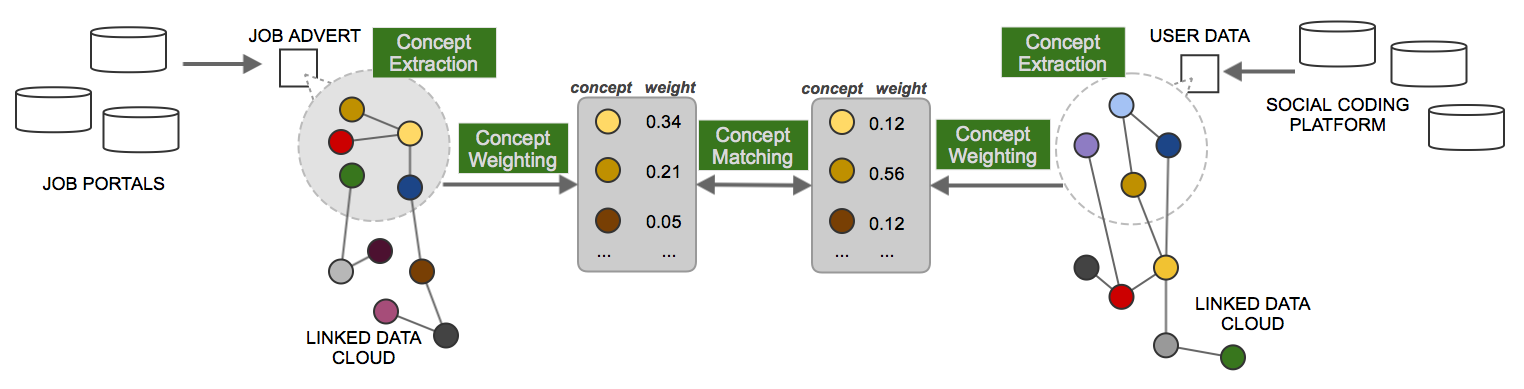
\includegraphics[scale=0.35]{images/pipeline.png}
\caption{Overview of our pipeline}
\label{fig:pipeline}
\end{figure*}

Today, social coding platforms have become an important tool for developers to showcase their work and become visible in the developer community. GitHub\footnote{\url{https://github.com/}} in particular has become an established way for developers to create a portfolio of their work to be considered during the hiring process by potential employers~\cite{dabbish2012social}. In order to find potential employers, developers search for job openings in various online job portals and compare their desires, experiences and activities with the described position. This is a cumbersome process as many job advertisements are lengthy, mentioning a plethora of programming languages, libraries and techniques that the perfect candidate should be familiar with.  Moreover, each of these items is usually conditioned on the number of years of experience or the level of expertise and may fall into the ``required'' or ``preferred'' skill category. Over the years, job advertisements have asked for a larger number of skills from prospective employees. This has led to a situation where a developer matching half of the described requirements may actually be a very well qualified candidate for the advertised position. In such cases having insights into how well other potential candidates fit the position may help the developer to judge whether to apply or not. Another complicating factor is the fact that job advertisements' writing style may be influenced by the numerous people involved in the creation of a job profile (managers, developers, HR personnel, etc.). Here a ``semantic gap'' may exist between search terms a developer is using to find suitable advertisements in job portals and the terms that actually appear in an advertisement. 

Similarly, judging the qualification of an applicant based on his or her GitHub profile is equally challenging~\cite{Singer:2013:MAS:2441776.2441791}. GitHub provides several user-based summary statistics such as \emph{Contributions in the last year}, \emph{Number of forked projects}, \emph{Number of followers}, however, the usefulness of this information is very limited, as it does not offer immediate insights into the developer's programming abilities, the particular languages the developer is regularly using or the type of development toolchain the developer is using. 
Marlow et al.~\cite{Marlow:2013:ATS:2441776.2441794} investigated how more detailed publicly accessible signals about a developer's activites on GitHub are used by employers in the recruitment process. In an interview-based study with several IT employers (active in the open-source community) they identified four main insights that employers can \emph{reliably} gain from a study of developer GitHub profiles: (1) Shared open source values, (2) Community acceptance of work \& contribution quality, (3) Project management skills, and (4) Passion for coding. Though again, the limiting factor in this setup is the time required to manually inspect each developer's profile.

Business-oriented social networks such as LinkedIn\footnote{\url{https://www.linkedin.com/}} are using recommender engines to \emph{push} job advertisements to its users (in addition to the traditional \emph{pull}-based model where users are actively searching among the available advertisements). Recommender algorithms determine the \emph{similarity} between pairs of user and advertisement profiles and recommend the job to the user if the similarity is high. While this process moves the burden of determining the degree of matching away from the user, it is limited in its abilities due to the lack of detailed user profile data as statements such as ``Experienced Java developer'' or ``Embedded Software Engineer'' contain relatively little information.

We conclude that considering the vast amounts of job advertisements in the IT sector (as well as the large number of developers), finding a job advertisement that is a good match with one's own abilities and desires is currently an inefficient process and likewise, determining how well an applicant from a group of applicants matches the position based on available GitHub user data is cumbersome and time-consuming. At the same time though, GitHub user data provides detailed insights that are not possible to be gained from other social Web sources.

In this paper we propose a pipeline that \emph{automatically} mines GitHub user profiles and job advertisements for relevant information. We employ an approach that ``translates'' both the developer profile and the advertisement into the Linked Open Data (LOD)~\cite{bizer2009linked} space, where we can exploit the background information available in the LOD cloud to bridge the semantic gap mentioned earlier. Additionally, this setup allows us to (partially) rely on well-tested algorithms and toolkits and it provides a natural mechanism to determine the similarity between a natural language job advertisement and a developer's GitHub profile. 

In the following section we describe our proof-of-concept and provide an overview of the challenges that need to be overcome.

A number of applications can benefit from this pipeline, including:
\begin{itemize}
\item ...
\item ...
\end{itemize}



\section{Approach}

The general overview of our pipeline is shown in Figure~\ref{fig:pipeline} with the three main components being:
\begin{itemize}
	\item \textbf{Extraction} of concepts from job advertisements and social coding user data
	\item \textbf{Weighting} of concepts in such a way that more important concepts receive higher weights
	\item \textbf{Matching} of the two (job and coding profile-based) concept vectors
\end{itemize}

On the left-hand side, we take as input a job advertisement in natural language text and extract the entities (or concepts) that appear in it. Named entity recognition (i.e. determining which word or phrase refers to some entity) in combination with named entity disambiguation (i.e. determining to which concrete entity a particular word/phrase refers to) have been shown to be powerful tools to turn natural language text into a more structured representation that machines can reason about. The three most commonly toolkits to annotate text are DBPedia Spotlight\footnote{\url{http://dbpedia-spotlight.github.io/}}, Open Calais\footnote{\url{http://www.opencalais.com/}} and AlchemyAPI\footnote{\url{http://www.alchemyapi.com/}}.

As a concrete example, consider this excerpt from one of the job advertisements in our data set. We annotated this text with DBPedia Spotlight, restricted the annotation to only those concepts of type \emph{computer} or \emph{internet}\footnote{More specifically, we restricted the types to belong to either \texttt{Freebase:/computer} or \texttt{Freebase:/internet}.}. Annotated are those phrases that are recognized as entities - 

\begin{quote}
The successful candidates will have experience of Object Oriented Programming \annotate{dbr/Object-oriented\_programming}  in at least one of PHP \annotate{dbr/PHP} (or another comparable, dynamic language), Java \annotate{dbr/Java\_(programming\_language)} (ideally with GWT \annotate{dbr/Google\_Web\_Toolkit}) or C++ \annotate{dbr/C++} (ideally with Win32 \annotate{Windows\_API}).
 
They will also be well versed in Test Driven Development and advanced practices of Object Oriented Programming such as Design Patterns and Refactoring.
\end{quote}

\section{Data}


We crawled XXX job advertisement in early 2015 containing the phrase \emph{Software Developer} from the UK version of the job portal Indeed\footnote{\url{http://www.indeed.co.uk}}. In total, $9,848$ job 


\subsection{Developer profiles}

Mining developer profiles from GitHub's publicly available data sources incurs the challenge of how to derive features from this raw data that are useful in the context of matching job advertisements to developers. Prior work has considered a number of high-level concepts that recruiters consider when looking for developers, such as ....

\subsection{Job profiles}

\subsection{Matching developer and job profiles}


\section{Preliminary Work}

\section{Related Work}

\section{Conclusions}

\bibliographystyle{IEEEtran}
\bibliography{dev-profiles}


\end{document}
